%Reproducing existing work with more languages
%New approach: based on par2vec (2 flavors)

We conducted several experiments using the multilingual \texttt{paragraph2vec} models described in~\ref{s:sentenceEmbeddings}. In this section, the training data and implementations we use are explained. We report emperical results for different experimental set-ups.



\subsection{Data}
% parallel 7x!! no pivot!!1! wow

For training the sentence and word embeddings, we use either of two subsets of the Europarl corpus.
The default training set contains 500 000 lines of Europarl data.
Another set has 50 000 lines that are sentence-aligned across English, German, Dutch, French, Spanish, Italian, and Portuguese.
These cross-lingual sentence alignments were created by matching the English side of all pairwise aligned corpora.
We use this dataset to train the multilingual dbow model in more than two languages, without making use of a pivot language.

All documents were tokenized and lowercased. No other preprocessing, such as stemming, was applied.
All words (and sentences) are represented by vectors of length 256.
In all experiments, words that occurred fewer than five times were excluded.
The resulting vocabulary sizes in these datasets are presented  in table~\ref{t:vocabularies}.

\begin{table}[ht]
\center
\begin{tabular}{l| r r}
		&Europarl 50k 	&Europarl 500k\\\hline
English	&8377			&24403	\\	
German	&11578		&47071	\\
Dutch		&10008				\\
French	&11092				\\	
Spanish	&10865				\\
Italian		&11503				\\
Portuguese	&11101				\\
\end{tabular}
\caption{Vocabulary size for Europarl data using a rare word cut-off of 5.}
\label{t:vocabularies}
\end{table}


As a baseline, we use the majority class estimate for the RCV data, and the F1 baseline $P$ explained in section~\ref{s:evaluation}. We also compare to the performance of vectors that results from the multitask-learning approach by \cite{klementiev2012inducing} described in section~\ref{s:relatedWork}. A distribution of their word embeddings in four language pairs (German-English, Czech-English, French-English, and Spanish-English) is available on \url{http://klementiev.org/data/distrib/}. The alignments used to populate the interaction matrix are obtained from the Europarl corpus. The word embeddings of the German-English part of the data are trained on the Reuters data that also make up the RCV evaluation set. Note that both the amount and nature of this training data differs from ours. Because of this, also the vocabularies differ. Their vocabulary size for English and German are 43612 and 50108, respectively. Since he I-Matrix vectors that we use are induced from RCV data, they fit better with that evaluation set. Also the length of these vectors is much smaller: 40 (instead of 256).



\subsection{Implementation}
%GENSIM tralala

All our experiments were run using the \texttt{gensim}\footnote{\url{https://github.com/piskvorky/gensim}} library.
The initial experiments were done by manually inspecting the nearest neighbours for selected words and sentences, and once the model was deemed sensible, we ran the evaluation pipeline.
The evalution was done with the setup from \cite{klementiev2012inducing}.
The code for experiments and evaluation is available online\footnote{\url{https://github.com/Veldhoen/mulidise}}.



\subsection{Sentence embeddings from multilingual dbow}
\begin{table*}[htb]
\center
\begin{tabular}{c | r|r r r r }
Sentences 		&		&	\multicolumn{4}{c}{Classification [train]-[test]}	\\
trained on: 		&paragraphs	&EN-EN	&DE-DE	&DE-EN	&EN-DE		\\\hline
EN			&.340		&.274		&.286		&.305		&.284		\\
DE			&.354		&.263		&.190		&.166		&.270		\\
DE-EN			&.363		&.319		&.304		&.264		&.323		\\
\end{tabular}
\caption{F1 scores on TED classification task for sentence representations (paragraphs) and word representations (parawords).}
\label{t:dbow_mono_bi}
\end{table*}

Using our multilingual version of the paragraph2vec dbow architecture, we obtain sentence embeddings for parallel sentences: DE-EN are German and English paired. EN and DE are monolingually trained sentence embeddings trained with the original dbow model. In each case, the model is trained on Europarl data, for 10 epochs. We start with a learning rate ($\alpha$) of 0.025, which is decreased with 0.002 after each epoch.

 In order to evaluate the quality of the sentence embeddings, we obtain sentence representations for the (parallel) TED corpus. We use the trained model, keeping the softmax weights fixed and training the TED sentence representations for 10 iterations.

We apply the induced sentence embeddings to the TED document classification task. In this case, we take the document representation to simply be the average of its sentence embeddings. These representations are then used to train and test the two document classification tasks. The results are in the second column of table~\ref{t:dbow_mono_bi}. 




\subsection{Word embeddings from sentence embeddings}

As explained in section~\ref{s:wordEmbeddings}, we obtain word embeddings from the sentence embeddings by taking the average of all sentence embeddings the word occurs in. We will refer to this setting as `parawords'. Note that we use only the Europarl-trained sentences for this, not the TED sentences that we reported on above. Again, we use sentences trained on English and German monolingually, as well as paired. The results are reported in the four rightmost columns table~\ref{t:dbow_mono_bi}.

Although the sentence representations trained on German perform somewhat better than those trained on English, the word representations induced from the latter appear much more useful for the document classification. Note that this is the case even for training/ testing on German document representations. In this case, the information from the English sentences is transferred to the German words. That means that the model might be trained monolingually on sentences in one language for which many data are available, and can be transferred to create word embeddings for other languages using a, possibly smaller, amount of parallel data.

The bilingually trained sentence representations yield better word representations than the monolingual ones in three of the four evaluation settings, which can be explained in there being more data available. However, the performance of sentence representations increases only slightly in the bilingual case.

We can also infer from these numbers that, apparently, monolingual classification is not necessarily `easier' than the cross-lingual case.





\begin{table}[ht]
\center
\setlength\tabcolsep{2pt}
\begin{tabular}{l | r r r r}
		& \multicolumn{4}{c}{Classification [train]-[test]}	\\
		&EN-EN	&DE-DE	&EN-DE	&DE-EN	\\\hline
Majority	&.468		&.468		&.468		&.468		\\
I-matrix	&.817		&.570		&.524		&.621		\\
Paraword  	&.837		&.694		&.656		&.748		\\
\end{tabular}
\caption{Accuracy score on RCV evaluation task with 1000 training documents, for word representations from I-matrix training and our own model trained on English-German parallel data.}
\label{t:dbow_bi_klemen}
\end{table}

In table~\ref{t:monoEval}, we report performance of the discussed experimental settings on monolingual (EN-EN) classification, to get an idea of how fit the different approaches are for the evaluation tasks. We report performance on the RCV task, again given 1000 training examples, TED, and the analogy task. The Google News vectors are provided in %???
They are English embeddings of length 300 and trained on a huge corpus (Google News). We reckon their performance therefore establishes an upper limit.

\begin{table}[ht]
\center
\setlength\tabcolsep{3pt}
\begin{tabular}{l |rr r r}
 			&vector	&RCV 			&TED		&Analogy\\
Setting		&length	&acc			&F1		&acc\\\hline
Baseline		&		&.468			&.118	 	&		\\
I-Matrix		&40		&.817			&.149		&.006\\
Paragraph e		&256		&- 			&.340		&-\\
Paragraph e-d 	&256		&- 			&.363		&-\\
Paraword e		&256		&.836			&.274		&.025	\\
Paraword e-d	&256		&.837			&.319		&.072\\
%Paraword multi 	&256		&\\	
Google News		&300		&.915			&.486		&.613\\
\end{tabular}
\caption{Monolingual (EN-EN) evaluation for various settings.
RCV Accuracy: given 1000 training examples for classification.}
\label{t:monoEval}
\end{table}

\subsection{Adding more languages}
As mentioned before, the multilingual dbow model can be trained for a larger number of languages at the same time. The precondition however, is to have sentence-aligned text for all those languages at the same time. We train on such data in seven languages, and create the word embeddings for each language in the same manner as before. We run the evaluation in all combinations of train and test data (TED). The results are shown in table~\ref{t:dbow_multi}. 
%We can see very clearly that 

\begin{table}[ht]
\center
\setlength\tabcolsep{3pt}
\begin{tabular}{l rrrrrrr}
&	de&	en&	nl&	es&	fr&	it&	pb\\
de&	\cca{.368}{37}&	\cca{.339}{34}&	\cca{.403}{40}&	\cca{.368}{37}&	\cca{.282}{28}&	\cca{.373}{37}&	\cca{.319}{32}\\
en&	\cca{.387}{39}&	\cca{.404}{40}&	\cca{.389}{39}&	\cca{.321}{32}&	\cca{.352}{35}&	\cca{.374}{37}&	\cca{.351}{35}\\
nl&	\cca{.426}{43}&	\cca{.397}{40}&	\cca{.417}{42}&	\cca{.393}{39}&	\cca{.412}{41}&	\cca{.428}{43}&	\cca{.321}{32}\\
es&	\cca{.399}{40}&	\cca{.301}{30}&	\cca{.428}{43}&	\cca{.387}{39}&	\cca{.354}{35}&	\cca{.362}{36}&	\cca{.355}{36}\\
fr&	\cca{.398}{40}&	\cca{.417}{42}&	\cca{.545}{54}&	\cca{.407}{41}&	\cca{.385}{38}&	\cca{.332}{33}&	\cca{.406}{41}\\
it&	\cca{.406}{41}&	\cca{.405}{41}&	\cca{.377}{38}&	\cca{.436}{44}&	\cca{.373}{37}&	\cca{.4}{40}&	\cca{.359}{36}\\
pb&	\cca{.403}{40}&	\cca{.333}{33}&	\cca{.369}{37}&	\cca{.354}{35}&	\cca{.374}{37}&	\cca{.405}{41}&	\cca{.315}{31}\\
\end{tabular}
\caption{}
\label{t:dbow_multi}
\end{table}


We investigated how language relatedness could influence these results. We train the dbow system on either the Germanic langugages German, English and Dutch (`G') or the Romance languages French, Spanish and Italian (`R'). 

We report the average over all evaluation settings with training/ testing on Germanic and Latin languages in table~\ref{t:dbow_families}. There is no apparent correlation between the language families of dbow training and evaluation.

\begin{table}[ht]
\center
\setlength\tabcolsep{2pt}
\begin{tabular}{l | r r r r}
		&G-G	&R-R	&R-G	&G-R	\\\hline
Germanic		&.338		&.374		&.383		&.349		\\
Romance		&.348		&.371		&.364		&.347		\\
\end{tabular}
\caption{F1 scores for classification on TED ([train]-[test])}
\label{t:dbow_families}
\end{table}



\subsection{Visualization}

As an illustration of the multilingual vector space, we present a visualization in figure~\ref{f:weekdays}.
We ran the word embeddings for the days of the week through the t-SNE optimization-based dimensionality reduction algorithm \cite{van2008visualizing}.
It is interesting to note that Saturday and Sunday are easily separable from the other days.
The fact that Portugese (in pink) uses words with multiple senses is also clearly visible.

\begin{figure}
\center
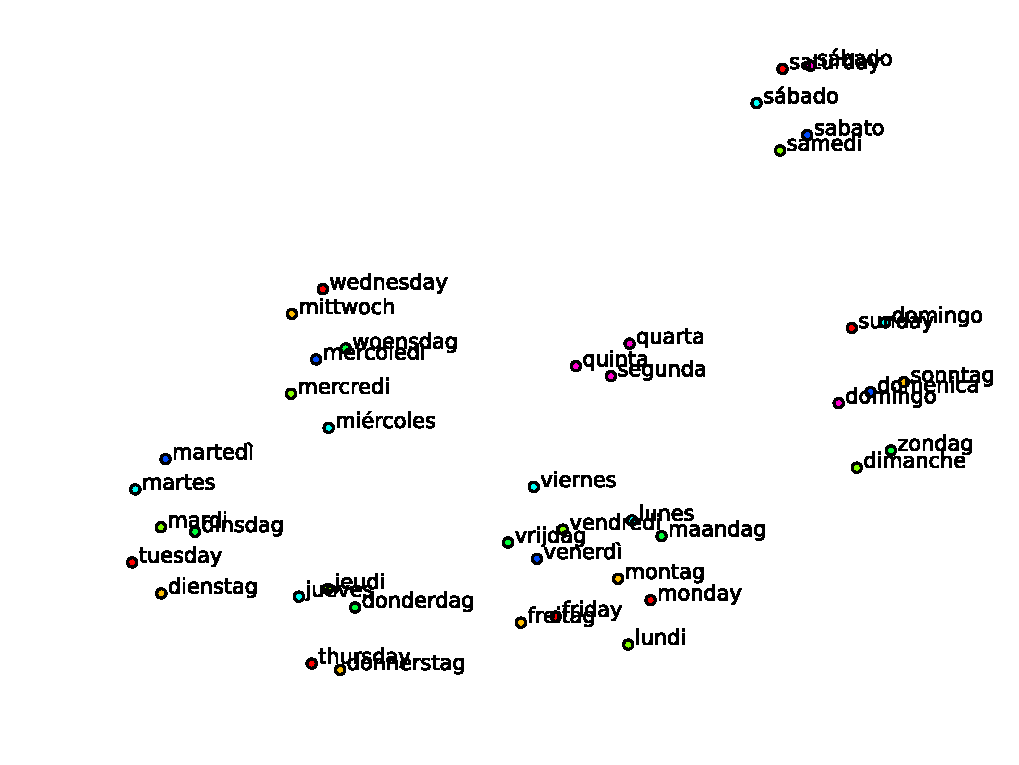
\includegraphics[width=1\linewidth]{figures/weekdays7}
\caption{Days of the week for 7 languages (if the words are present in the vocabulary)}
\label{f:weekdays}
\end{figure}
